\documentclass[12pt,english,ignorenonframetext,aspectratio=169,]{beamer}


%%%%%%%%%%%%%%%
%% Beamer theme
% choose one from http://deic.uab.es/~iblanes/beamer_gallery/
% or http://www.hartwork.org/beamer-theme-matrix/
% \usetheme{Warsaw}
\usetheme{CambridgeUS}

%%%%%%%%%%%%%%%%%%%%%%
%% Beamer color theme
%% default albatross beaver beetle crane dolphin dove fly lily
%% orchid rose seagull seahorse whale wolverine

%\usecolortheme{seahorse}  %% very lighty
\usecolortheme{dolphin}    %% nice blue
\usecolortheme{orchid}     %% dark red ?
\usecolortheme{whale}      %% black and blue as Warsaw

%%%%%%%%%%%%%%%%%%%%%%%%%%%%%%%%%%%%%%%%%%%%%%%%%%%%%%%%%%%%%%%%%%%%%%%%%%%%%%%%
%% Define your own colors
\definecolor{blackblue}{rgb}{19,19,59}  % rgb(48,48,150)

%%%%%%%%%%%%%%%%%%%%%%%%%%%%%%%%%%%%%%%%%%%%%%%%%%%%%%%%%%%%%%%%%%%%%%%%%%%%%%%%
%% Change the theme
%\setbeamercolor{alerted text}{fg=orange}
%\setbeamercolor{background canvas}{bg=white}
%\setbeamercolor{block body alerted}{bg=normal text.bg!90!black}
%\setbeamercolor{block body}{bg=normal text.bg!90!black}
%\setbeamercolor{block body example}{bg=normal text.bg!90!black}
%\setbeamercolor{block title alerted}{use={normal text,alerted text},fg=alerted text.fg!75!normal text.fg,bg=normal text.bg!75!black}
%\setbeamercolor{block title}{bg=blue}
%\setbeamercolor{block title example}{use={normal text,example text},fg=example text.fg!75!normal text.fg,bg=normal text.bg!75!black}
%\setbeamercolor{fine separation line}{}
\setbeamercolor{frametitle}{fg=black}
%\setbeamercolor{item projected}{fg=black}
%\setbeamercolor{normal text}{bg=black,fg=yellow}
%\setbeamercolor{palette sidebar primary}{use=normal text,fg=normal text.fg}
%\setbeamercolor{palette sidebar quaternary}{use=structure,fg=structure.fg}
%\setbeamercolor{palette sidebar secondary}{use=structure,fg=structure.fg}
%\setbeamercolor{palette sidebar tertiary}{use=normal text,fg=normal text.fg}
%\setbeamercolor{section in sidebar}{fg=brown}
%\setbeamercolor{section in sidebar shaded}{fg= grey}
\setbeamercolor{separation line}{}
%\setbeamercolor{sidebar}{bg=red}
%\setbeamercolor{sidebar}{parent=palette primary}
%\setbeamercolor{structure}{bg=black, fg=green}
%\setbeamercolor{subsection in sidebar}{fg=brown}
%\setbeamercolor{subsection in sidebar shaded}{fg= grey}
%\setbeamercolor{title}{fg=blackblue}
%\setbeamercolor{titlelike}{fg=blackblue}


%%%%%%%%%%%%%%%%%%%%%%%
%% Other beamer options
%\setbeamercovered{transparent}
% Permet de laisser en gris le texte qui n'est pas encore apparu (lorsqu'on utilise les commandes avec des <1,2> ou <4-9>.

%\setbeamercolor{normal text}{fg=black,bg=white}

%%%%%%%%%%%%%%%%%%%%%%%
%% Change Beamer fonts
% \usefonttheme{default}
% \usefonttheme[onlymath]{serif}
\usefonttheme{serif}

\setbeamerfont{title}{family=\rm}
\setbeamerfont{titlelike}{family=\rm}
\setbeamerfont{frametitle}{family=\rm}

%%%%%%%%%%%%%%%%%%%%%%%%%%%%%%%%%%%%%%%%%%%%%%%%%%%%%%%%%%%%%%%%%%%%%%%%%%%%%%%%
%% innertheme
%% rectangles circles inmargin rounded
% \useinnertheme{rounded}  % XXX My preference
\useinnertheme{circles}    % XXX

%%%%%%%%%%%%%%%%%%%%%%%%%%%%%%%%%%%%%%%%%%%%%%%%%%%%%%%%%%%%%%%%%%%%%%%%%%%%%%%%
%% outertheme
%% infolines miniframes shadow sidebar smoothbars smoothtree split tree
%\useoutertheme{infolines}

%% No navigation symbol.
\setbeamertemplate{navigation symbols}{}
\beamertemplatenavigationsymbolsempty

% XXX Add a background image to the slides
\usepackage{tikz}
% \setbeamertemplate{background}{
\includegraphics[width=\paperwidth,height=\paperheight,keepaspectratio]{IETR.jpg}}
% \setbeamertemplate{background}{{\centering\begin{tikzpicture}\node[opacity=0.15]{
\includegraphics[width=0.98\paperwidth]{IETR_et_partenaires_IETR.png}};\end{tikzpicture}}}

% Other options
%\setbeamertemplate{footline}[page number]

\beamertemplateballitem
\setbeamertemplate{itemize item}[square]


\setbeamertemplate{caption}[numbered]
\setbeamertemplate{caption label separator}{: }
\setbeamercolor{caption name}{fg=normal text.fg}
\beamertemplatenavigationsymbolsempty
\usepackage{lmodern}
\usepackage{color}
  \newcommand{\urlb}[1]{\textcolor{blue}{\url{#1}}}
\usepackage{amssymb,amsmath}
\usepackage{ifxetex,ifluatex}
\usepackage{fixltx2e} % provides \textsubscript

\ifnum 0\ifxetex 1\fi\ifluatex 1\fi=0 % if pdftex
  \usepackage[T1]{fontenc}
  \usepackage[utf8]{inputenc}
\else % if luatex or xelatex
  \ifxetex
    \usepackage{mathspec}
  \else
    \usepackage{fontspec}
  \fi
  \defaultfontfeatures{Ligatures=TeX,Scale=MatchLowercase}
\fi
% use upquote if available, for straight quotes in verbatim environments
\IfFileExists{upquote.sty}{\usepackage{upquote}}{}
% use microtype if available
\IfFileExists{microtype.sty}{%
\usepackage{microtype}
\UseMicrotypeSet[protrusion]{basicmath} % disable protrusion for tt fonts
}{}
\ifnum 0\ifxetex 1\fi\ifluatex 1\fi=0 % if pdftex
  \usepackage[shorthands=off,main=english]{babel}
\else
  \usepackage{polyglossia}
  \setmainlanguage[]{}
\fi
\newif\ifbibliography
\hypersetup{
            pdftitle={MAB Learning in IoT Networks},
            pdfauthor={Lilian Besson, Rémi Bonnefoi, Émilie Kaufmann, Christophe Moy, Jacques Palicot},
            pdfborder={0 0 0},
            breaklinks=true}
% \urlstyle{same}  % don't use monospace font for urls
% Code embedding.
\usepackage{palatino}              % Use the Palatino font % XXX remove if it is ugly ?

% Prevent slide breaks in the middle of a paragraph:
\widowpenalties 1 10000
\raggedbottom


\setlength{\parindent}{0pt}
\setlength{\parskip}{6pt plus 2pt minus 1pt}
\setlength{\emergencystretch}{3em}  % prevent overfull lines
\providecommand{\tightlist}{%
  \setlength{\itemsep}{0pt}\setlength{\parskip}{0pt}}
\setcounter{secnumdepth}{5}

  \title{MAB Learning in IoT Networks}
  \subtitle{Learning helps even in non-stationary settings!}
    \author[Lilian Besson]{\textbf{Lilian Besson} \and Rémi Bonnefoi \newline
\and Émilie Kaufmann \and Christophe Moy \and Jacques Palicot}
        \institute[CentraleSupélec \& Inria]{PhD Student in France \newline Team SCEE, IETR, CentraleSupélec, Rennes
\newline \& Team SequeL, CRIStAL, Inria, Lille}
        \date[CROWNCOM 2017]{20-21 Sept - CROWNCOM 2017}

% For \justifying command, see https://tex.stackexchange.com/a/148696/
\usepackage{ragged2e}
\addtobeamertemplate{frame begin}{}{\justifying}
\addtobeamertemplate{block begin}{}{\justifying}
\addtobeamertemplate{block alerted begin}{}{\justifying}
\addtobeamertemplate{block example begin}{}{\justifying}
\addtobeamertemplate{itemize body begin}{}{\justifying}
\addtobeamertemplate{itemize item}{}{\justifying}
\addtobeamertemplate{itemize subitem}{}{\justifying}
\addtobeamertemplate{itemize subsubitem}{}{\justifying}
\addtobeamertemplate{enumerate body begin}{}{\justifying}
\addtobeamertemplate{enumerate item}{}{\justifying}
\addtobeamertemplate{enumerate subitem}{}{\justifying}
\addtobeamertemplate{enumerate subsubitem}{}{\justifying}
\addtobeamertemplate{description body begin}{}{\justifying}
\addtobeamertemplate{description item}{}{\justifying}

\begin{document}
\justifying

\begin{frame}[plain]
\titlepage

% XXX manual inclusion of logos
\begin{center}

\includegraphics[height=0.13\textheight]{../common/LogoIETR.png}

\includegraphics[height=0.13\textheight]{../common/LogoCS.png}

\includegraphics[height=0.13\textheight]{../common/LogoInria.jpg}
\end{center}

\end{frame}

\section*{\hfill{}CentraleSupélec Rennes \& Inria Lille\hfill{}}

\subsection*{\hfill{}Team {:} SCEE @ IETR \& SequeL @ CRIStAL\hfill{}}




\section{\hfill{}1. Introduction and motivation\hfill{}}

\subsection{\hfill{}1.a. Objective\hfill{}}

\begin{frame}{We want}
A \emph{lot} of IoT devices want to access to a gateway of base station.

\begin{itemize}
\tightlist
\item
  Insert them in a \textbf{crowded wireless network}.
\item
  With a protocol \textbf{slotted in time and frequency}.
\item
  Each device has a \textbf{low duty cycle} (a few messages per day).
\end{itemize}

\pause

\begin{block}{Goal}

\begin{itemize}
\tightlist
\item
  Maintain a \textbf{good Quality of Service}.
\item
  \textbf{Without} centralized supervision!
\end{itemize}

\end{block}

\pause

\begin{block}{How?}

\begin{itemize}
\tightlist
\item
  Use \textbf{learning algorithms}: devices will learn on which
  frequency they should talk!
\end{itemize}

\end{block}

\end{frame}



\subsection{\hfill{}1.b. Outline\hfill{}}

\begin{frame}{Outline}

\begin{enumerate}
\def\labelenumi{\arabic{enumi}.}
\tightlist
\item
  Introduction and motivation
\item
  Model and hypotheses
\item
  Baseline algorithms : to compare against naive and efficient
  centralized approaches
\item
  Multi-Armed Bandit algorithms : UCB
  % , Thompson sampling
\item
  Experimental results
\item
  Perspectives and future works
\item
  Conclusion
\end{enumerate}

\end{frame}



\section{\hfill{}2. Model and hypotheses\hfill{}}

\subsection{\hfill{}2.a. Model\hfill{}}

\begin{frame}{Model}

\begin{itemize}
\tightlist
\item
  Discrete time \(t\geq1\) and \(N_c\) radio channels (\emph{e.g.}, 10)
  \hfill{} (\emph{known})
\end{itemize}

\begin{figure}[h!]
\centering
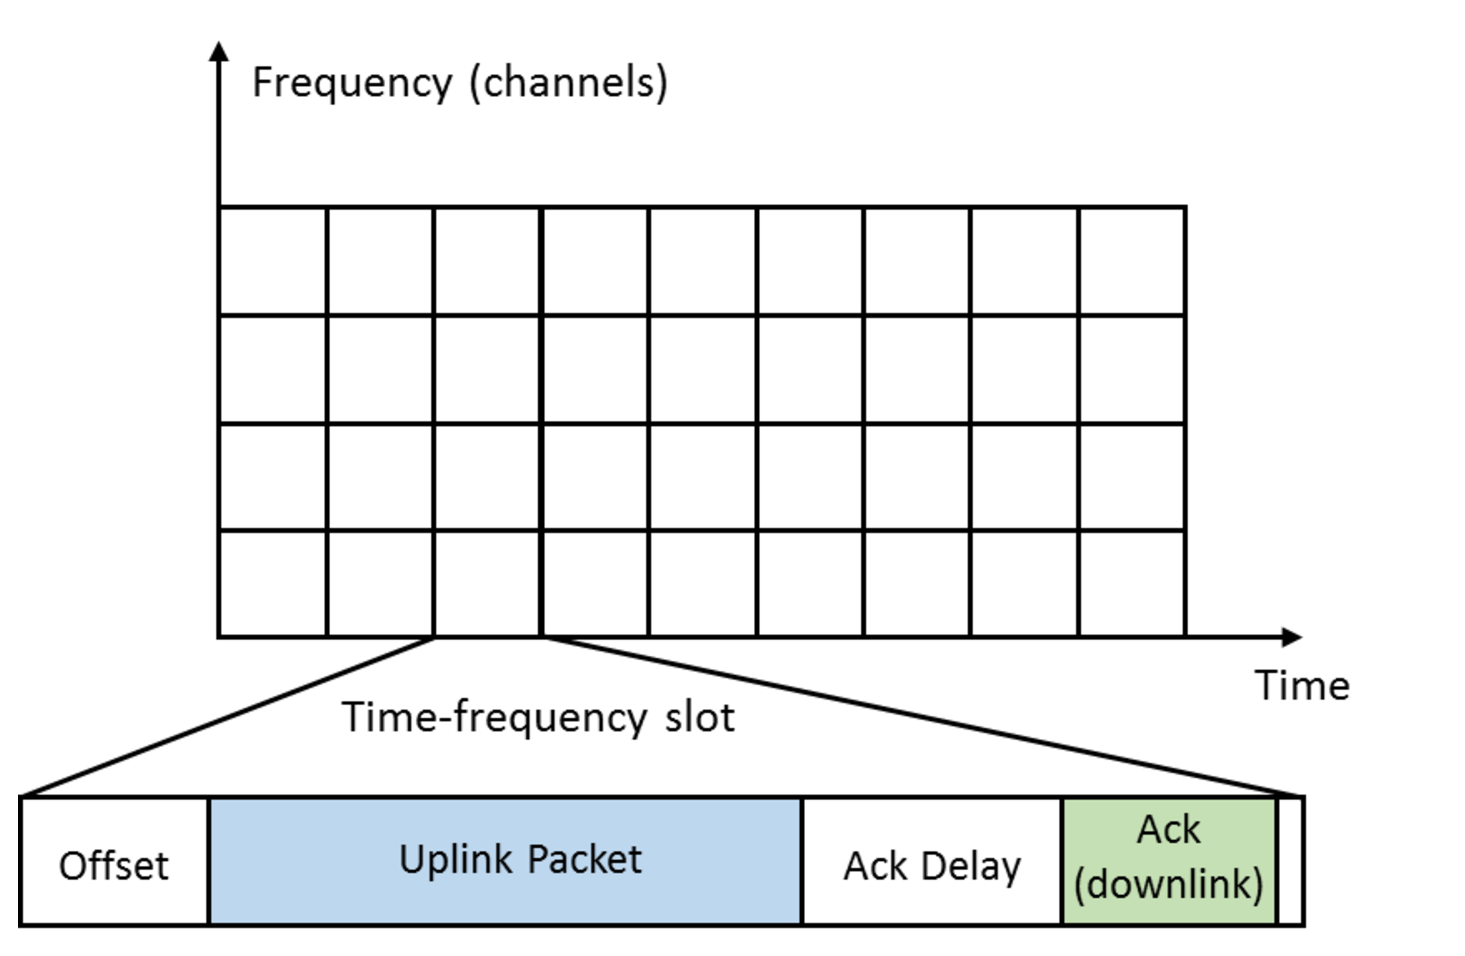
\includegraphics[height=0.35\textheight]{protocol.eps}
\caption{\small{Protocol in time and frequency, with an \emph{Acknowledgement}.}}
\end{figure}

\begin{itemize}
\tightlist
\item
  \(D\) \textbf{dynamic} devices try to access the network
  \emph{independently}
\item
  \(S=S_1+\dots+S_{N_c}\) \textbf{static} devices occupy the network :
  \newline
   \(S_1,\dots,S_{N_c}\) in each channel \hfill{} (\emph{unknown}).
\end{itemize}

\end{frame}



\subsection{\hfill{}2.b. Hypotheses\hfill{}}

\begin{frame}[fragile,allowframebreaks]{Hypotheses}

\begin{block}{Emission model}

\begin{itemize}
\tightlist
\item
  Each device has the same \emph{low} emission probability: \newline
   each step, each device sends a packet with probability \(p\).
  \newline
   \hfill{}\small{(this gives a duty cycle proportional to $1/p$)}
\end{itemize}

\end{block}

\begin{block}{Background traffic}

\begin{itemize}
\tightlist
\item
  Each static device uses only one channel.
\item
  Their repartition is fixed in time.
\end{itemize}

\end{block}

\begin{quote}
\(\implies\) Background traffic, bothering the dynamic devices!
\end{quote}

\begin{block}{Dynamic radio reconfiguration}

\begin{itemize}
\tightlist
\item
  Each \textbf{dynamic device decides the channel it uses to send every
  packet}.
\item
  It has memory and computational capacity to implement basic decision
  algorithm.
\end{itemize}

\end{block}

\begin{block}{Problem}

\begin{itemize}
\tightlist
\item
  \emph{Goal} : \emph{maximize packet loss ratio} (\(=\) number of
  received \texttt{Ack}) in a \emph{finite-space discrete-time Decision
  Making Problem}.
\item
  \emph{Solution ?} \textbf{Multi-Armed Bandit algorithms},
  \textbf{decentralized} and used \textbf{independently} by each device.
\end{itemize}

\end{block}

\end{frame}



\section{\hfill{}3. Baseline algorithms\hfill{}}

\subsection{\hfill{}3.a. A naive strategy : uniformly random access\hfill{}}

\begin{frame}{A naive strategy : uniformly random access}

\begin{itemize}
\tightlist
\item
  \textbf{Uniformly random access}: dynamic devices choose uniformly
  their channel in the pull of \(N_c\) channels.
\item
  Natural strategy, dead simple to implement.
\end{itemize}

\pause

\begin{itemize}
\tightlist
\item
  Simple analysis, in term of \textbf{successful transmission
  probability} (for every message from dynamic devices) :
\end{itemize}

\begin{small} \begin{align*}
\mathbb{P}(\text{success}|\text{sent}) = \sum_{i=1}^{N_c} \underbrace{(1 - p / N_c)^{D-1}}_{\text{No other dynamic device}} \times \underbrace{(1-p)^{S_i}}_{\text{No static device}} \times\; \frac{1}{N_c}.
\end{align*} \end{small}

\pause

\begin{itemize}
\tightlist
\item
  Works fine only if all channels are similarly occupied,\newline
   but \textbf{it cannot learn} to exploit the best (more free)
  channels.
\end{itemize}

\end{frame}



\subsection{\hfill{}3.b. Optimal centralized strategy\hfill{}}

\begin{frame}[allowframebreaks]{Optimal centralized strategy}

\begin{itemize}
\tightlist
\item
  If an oracle can decide to affect \(D_i\) dynamic devices to channel
  \(i\), the \textbf{successful transmission probability} is:
  \vspace*{-10pt}

  \begin{small} \begin{align*}
  \mathbb{P}(\text{success}|\text{sent}) = \sum_{i=1}^{N_c} \underbrace{(1 - p)^{D_i - 1}}_{\;\;D_i - 1 \;\text{others}\;\;} \times \underbrace{(1 - p)^{S_i}}_{\;\;\text{No static device}\;\;} \times \underbrace{ D_i / D }_{\;\;\text{Sent in channel}\; i}.
  \end{align*} \end{small}
\item
  The oracle has to solve this \textbf{optimization problem}:
  \vspace*{-5pt}

  \begin{small} \begin{equation*} \begin{cases}
  \underset{D_1,\dots,D_{N_c}}{\arg\max}\;\;\; & \sum_{i=1}^{N_c} D_i (1 - p)^{S_i + D_i -1}\\
  \text{such that}\;\;\; & \sum_{i=1}^{N_c} D_i = D \; \text{and} \; D_i \geq 0, \; \; \forall 1 \leq i \leq N_c .
  \end{cases} \end{equation*} \end{small}
\item
  We solved this quasi-convex optimization problem with \emph{Lagrange
  multipliers}, only numerically.
\item
  \(\implies\) Very good performance, maximizing the transmission rate
  of all the \(D\) dynamic devices
\end{itemize}

\begin{block}{But unrealistic}

But \textbf{not achievable in practice}: no centralized oracle!

\end{block}

\begin{block}{Let see \emph{realistic decentralized approaches}}

\(\hookrightarrow\) Machine Learning ? \newline
\hspace*{15pt}\(\hookrightarrow\) Reinforcement Learning ? \newline
\hspace*{30pt} \(\hookrightarrow\) \emph{Multi-Armed Bandit} !

\end{block}

\end{frame}



\section{\hfill{}4. Multi-Armed Bandit algorithm : UCB\hfill{}}

\subsection{\hfill{}4.1. Multi-Armed Bandit formulation\hfill{}}

\begin{frame}[fragile]{Multi-Armed Bandit formulation}

A dynamic device tries to collect \emph{rewards} when transmitting :

\begin{itemize}
\tightlist
\item
  it transmits following a Bernoulli process \newline
   (probability \(p\) of transmitting at each time step \(\tau\)),
\item
  chooses a channel \(A(\tau) \in \{1,\dots,N_c\}\),
\item
  if \texttt{Ack} (no collision) \hspace*{10pt} \(\implies\) reward
  \(r_{A(\tau)} = 1\),
\item
  if collision (no \texttt{Ack}) \hspace*{10pt} \(\implies\) reward
  \(r_{A(\tau)} = 0\).
\end{itemize}

\pause

\begin{block}{Reinforcement Learning interpretation}

Maximize transmission rate \(\equiv\) \textbf{maximize cumulated
rewards}
\[\max_{\text{algorithm}\;A} \;\; \sum_{\tau=1}^{\text{horizon}} r_{A(\tau)}.\]

\end{block}

\end{frame}

\subsection{\hfill{}4.2. Upper Confidence Bound algorithm : UCB\hfill{}}

\begin{frame}{Upper Confidence Bound algorithm (\(\mathrm{UCB}_1\))}

A dynamic device keeps \(\tau\) number of sent packets, \(T_k(t)\)
selections of channel \(k\), \(X_k(t)\) successful transmission in
channel \(k\).

\begin{enumerate}
\def\labelenumi{\arabic{enumi}.}
\tightlist
\item
  For the first \(N_c\) steps (\(\tau=1,\dots,N_c\)), try each channel
  \emph{once}.
\item
  Then for the next steps \(t \geq N_c\) :

  \begin{itemize}
  \tightlist
  \item
    Compute the index
    \(g_k(\tau) := \underbrace{\frac{X_k(\tau)}{N_k(\tau)}}_{\text{Mean}\; \widehat{\mu_k}(\tau)} + \underbrace{\sqrt{\frac{\log(\tau)}{2 N_k(\tau)}},}_{\text{Upper Confidence Bound}}\)
  \item
    Choose channel
    \(A(\tau) = \mathop{\arg\max}\limits_{k} \; g_k(\tau)\),
  \item
    Update \(T_k(\tau+1)\) and \(X_k(\tau+1)\).
  \end{itemize}
\end{enumerate}

\vfill{}\hfill{}\tiny{\textcolor{gray}{References: [Lai \& Robbins, 1985], [Auer et al, 2002], [Bubeck \& Cesa-Bianchi, 2012]}}

\end{frame}



\section{\hfill{}5. Experimental results\hfill{}}

\subsection{\hfill{}5.1. Experiment setting\hfill{}}

\begin{frame}{Experimental setting}

\begin{block}{Simulation parameters}

\begin{itemize}
\tightlist
\item
  \(N_c = 10\) channels,
\item
  \(S + D = 10000\) devices in total,
\item
  \(p = 10^{-3}\) probability of emission,
\item
  \(\text{horizon} = 10^5\) time slots (\(\simeq 100\) messages \(/\)
  device),
\item
  The proportion of dynamic devices \(D/(S+D)\) varies,
\item
  Various settings for \((S_1,\dots,S_{N_c})\) static devices
  repartition.
\end{itemize}

\end{block}

\begin{block}{What do we show}

\begin{itemize}
\tightlist
\item
  After a short learning time, MAB algorithms are almost as efficient as
  the oracle solution.
\item
  Never worse than the naive solution.
\item
  Thompson sampling is even more efficient than UCB.
\end{itemize}

\end{block}

\end{frame}



\subsection{\hfill{}5.2. First result: $10\%$\hfill{}}

\begin{frame}{\(10\%\) of dynamic devices}

\begin{figure}[h!]
\centering
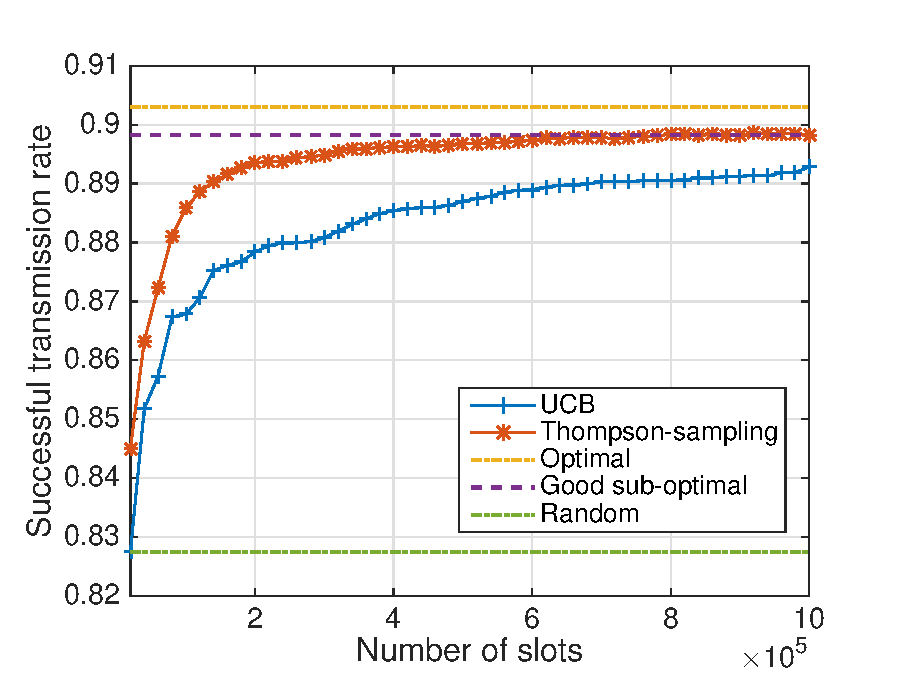
\includegraphics[height=0.74\textheight]{10intelligent.eps}
\caption{\small{$10\%$ of dynamic devices. $7\%$ of gain.}}
\end{figure}

\end{frame}



\subsection{\hfill{}5.2. First result: $30\%$\hfill{}}

\begin{frame}{\(30\%\) of dynamic devices}

\begin{figure}[h!]
\centering
\includegraphics[height=0.74\textheight]{30intelligent.eps}
\caption{\small{$30\%$ of dynamic devices.} $3\%$ of gain but not much is possible.}
\end{figure}

\end{frame}



\subsection{\hfill{}5.3. Growing proportion of devices dynamic devices\hfill{}}

\begin{frame}{Dependence on \(D/(S+D)\)}

\begin{figure}[h!]
\centering
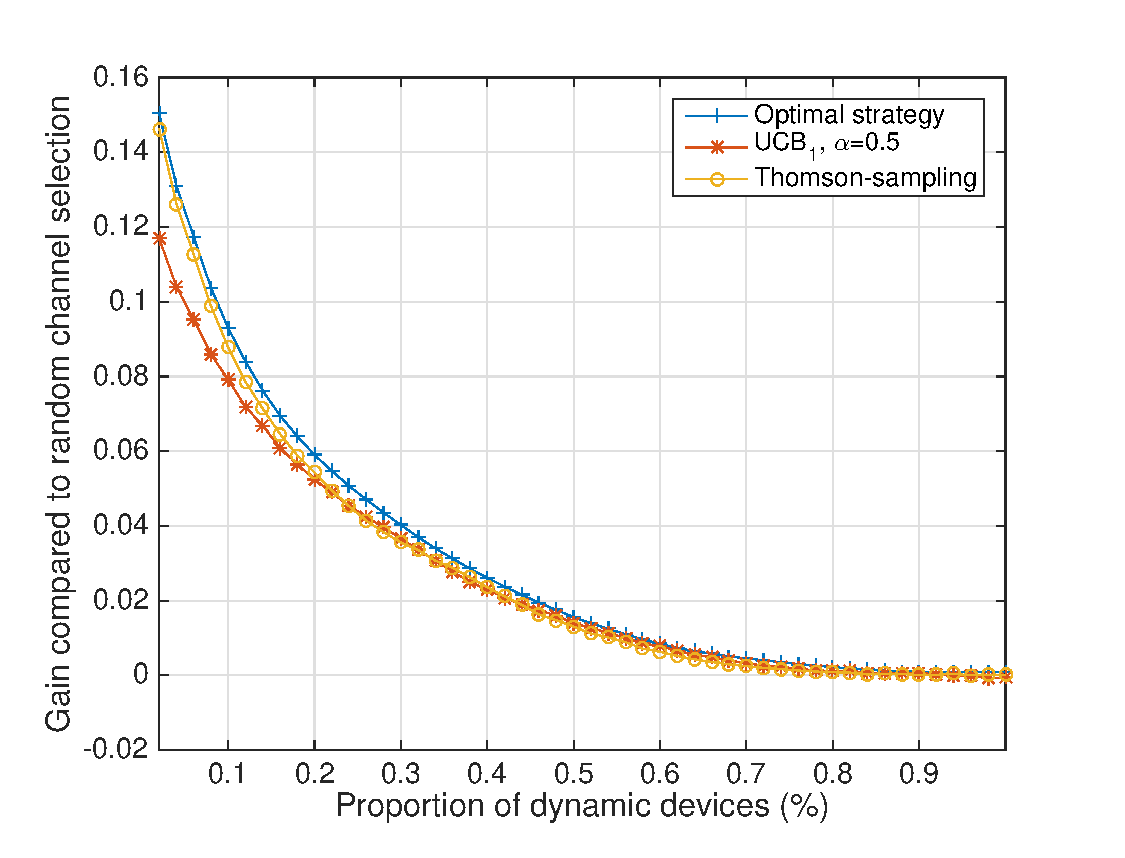
\includegraphics[height=0.65\textheight]{perf_learning.eps}
\caption{\small{\emph{Almost optimal}, for any proportion of dynamic devices, \emph{after a short learning time}. Up-to $16\%$ gain over the naive approach!}}
\end{figure}

\end{frame}



\section{\hfill{}6. Perspectives and future work\hfill{}}

\subsection{\hfill{}6.1. Perspectives\hfill{}}

\begin{frame}{Perspectives}

\begin{block}{Theoretical results}

\begin{itemize}
\tightlist
\item
  MAB algorithms have performance guarantees for \emph{stochastic
  settings},
\item
  But here the collisions cancel the \emph{i.i.d.} hypothesis,
\item
  Not easy to obtain guarantees in this mixed setting \newline
   (\emph{i.i.d.} emission process, game theoretic collisions).
\end{itemize}

\pause

\end{block}

\begin{block}{Real-world experimental validation ?}

\begin{itemize}
\tightlist
\item
  Real-world radio experiments will help to validate this. \newline
   \hspace*{40pt}\hfill{}\textcolor{gray}{In progress\dots}
\end{itemize}

\end{block}

\end{frame}



\subsection{\hfill{}6.2. Future work\hfill{}}

\begin{frame}{Other direction of future work}

\begin{itemize}
\item
  \emph{More realistic emission model}: maybe driven by number of
  packets in a whole day, instead of emission probability.
\item
  Validate this on a \emph{larger experimental scale}.
\end{itemize}

\end{frame}



\section{\hfill{}7. Conclusion\hfill{}}\subsection{\hfill{}Thanks!\hfill{}}

\begin{frame}{Conclusion}

\begin{block}{We showed numerically\ldots{}}

\begin{itemize}
\tightlist
\item
  After a learning period, MAB algorithms are as efficient as we could expect.
\item
  Never worse than the naive solution.
\item
  Thompson sampling is even more efficient than UCB.
\item
  Simple algorithms are up-to \(16\%\) more efficient than the naive
  approach, and straightforward to apply.
\end{itemize}

\end{block}

\begin{block}{But more work is still needed\ldots{}}

\begin{itemize}
\tightlist
\item
  \textbf{Theoretical guarantees} are still missing.
\item
  Maybe study \textbf{other emission models}.
\item
  And also implement this on \textbf{real-world radio devices}.
\end{itemize}

\end{block}

\hfill{} \textbf{Thanks!} \emph{Question?}

\end{frame}

\appendix
\backupbegin

\section{\hfill{}Appendix\hfill{}}

\subsection{\hfill{}A.1. Thompson Sampling : Bayesian index policy\hfill{}}

\begin{frame}[noframenumbering]{Thompson Sampling : Bayesian approach}

A dynamic device assumes a stochastic hypothesis on the background
traffic, modeled as Bernoulli distributions.

\begin{itemize}
\item
  Rewards \(r_k(\tau)\) are assumed to be \emph{i.i.d.} samples from a
  Bernoulli distribution \(\mathrm{Bern}(\mu_k)\).
\item
  A \textbf{binomial Bayesian posterior} is kept on the mean
  availability \(\mu_k\) :
  \(\mathrm{Bin}(1 + X_k(\tau), 1 + N_k(\tau) - X_k(\tau))\).
\item
  Starts with a \emph{uniform prior} :
  \(\mathrm{Bin}(1, 1) \sim \mathcal{U}([0,1])\).
\end{itemize}

\begin{enumerate}
\def\labelenumi{\arabic{enumi}.}
\tightlist
\setlength{\itemindent}{1em}  % https://stackoverflow.com/a/2612825/
\item
  Each step \(\tau \geq 1\), a sample is drawn from each posterior
  \(i_k(t) \sim \mathrm{Bin}(a_k(\tau), b_k(\tau))\),
\item
  Choose channel \(A(\tau) = \mathop{\arg\max}\limits_k \; i_k(\tau)\),
\item
  Update the posterior after receiving \texttt{Ack} or if collision.
\end{enumerate}

\vfill{}\hfill{}\tiny{\textcolor{gray}{References: [Thompson, 1933], [Kaufmann et al, 2012]}}

\end{frame}

\backupend

\end{document}
